\begin{figure}[H]
	\centering
	\begin{tabular}{cc}
		\centering
		{\scriptsize 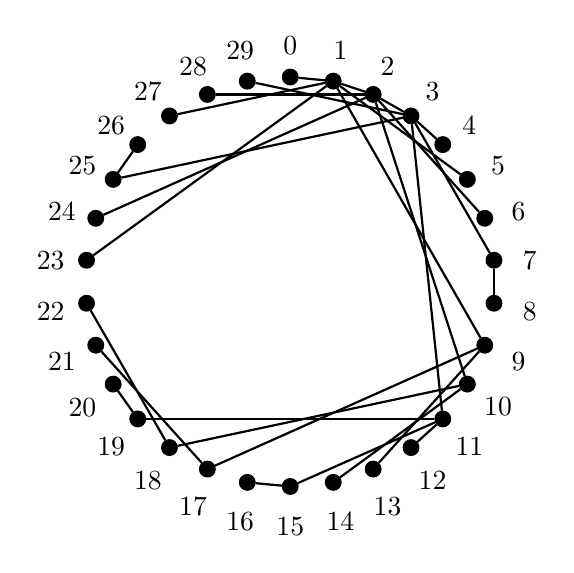
\begin{tikzpicture}
	\tikzset{enclosed/.style={draw, circle, inner sep=0pt, minimum size=0.2cm, fill=black}}

	\node[enclosed, label={above, xshift=0cm, yshift=0.052cm:0}] at (3.38, 5.2)(0){};
	\node[enclosed, label={above, xshift=0.091cm, yshift=0.039cm:1}] at (3.926, 5.148)(1){};
	\node[enclosed, label={above, xshift=0.182cm, yshift=0.013cm:2}] at (4.433, 4.979)(2){};
	\node[enclosed, label={above, xshift=0.273cm, yshift=-0.039cm:3}] at (4.914, 4.706)(3){};
	\node[enclosed, label={above, xshift=0.338cm, yshift=-0.104cm:4}] at (5.317, 4.342)(4){};
	\node[enclosed, label={above, xshift=0.39cm, yshift=-0.169cm:5}] at (5.629, 3.9)(5){};
	\node[enclosed, label={above, xshift=0.429cm, yshift=-0.26cm:6}] at (5.85, 3.406)(6){};
	\node[enclosed, label={above, xshift=0.455cm, yshift=-0.351cm:7}] at (5.967, 2.873)(7){};
	\node[enclosed, label={above, xshift=0.455cm, yshift=-0.455cm:8}] at (5.967, 2.327)(8){};
	\node[enclosed, label={above, xshift=0.429cm, yshift=-0.546cm:9}] at (5.85, 1.794)(9){};
	\node[enclosed, label={above, xshift=0.39cm, yshift=-0.624cm:10}] at (5.629, 1.3)(10){};
	\node[enclosed, label={above, xshift=0.338cm, yshift=-0.702cm:11}] at (5.317, 0.858)(11){};
	\node[enclosed, label={above, xshift=0.273cm, yshift=-0.767cm:12}] at (4.914, 0.494)(12){};
	\node[enclosed, label={above, xshift=0.182cm, yshift=-0.819cm:13}] at (4.433, 0.221)(13){};
	\node[enclosed, label={above, xshift=0.091cm, yshift=-0.845cm:14}] at (3.926, 0.052)(14){};
	\node[enclosed, label={above, xshift=0cm, yshift=-0.858cm:15}] at (3.38, 0)(15){};
	\node[enclosed, label={above, xshift=-0.091cm, yshift=-0.845cm:16}] at (2.834, 0.052)(16){};
	\node[enclosed, label={above, xshift=-0.182cm, yshift=-0.819cm:17}] at (2.327, 0.221)(17){};
	\node[enclosed, label={above, xshift=-0.273cm, yshift=-0.767cm:18}] at (1.846, 0.494)(18){};
	\node[enclosed, label={above, xshift=-0.338cm, yshift=-0.702cm:19}] at (1.443, 0.858)(19){};
	\node[enclosed, label={above, xshift=-0.39cm, yshift=-0.637cm:20}] at (1.131, 1.3)(20){};
	\node[enclosed, label={above, xshift=-0.429cm, yshift=-0.546cm:21}] at (0.91, 1.794)(21){};
	\node[enclosed, label={above, xshift=-0.455cm, yshift=-0.455cm:22}] at (0.793, 2.327)(22){};
	\node[enclosed, label={above, xshift=-0.455cm, yshift=-0.351cm:23}] at (0.793, 2.873)(23){};
	\node[enclosed, label={above, xshift=-0.429cm, yshift=-0.26cm:24}] at (0.91, 3.406)(24){};
	\node[enclosed, label={above, xshift=-0.39cm, yshift=-0.169cm:25}] at (1.131, 3.9)(25){};
	\node[enclosed, label={above, xshift=-0.338cm, yshift=-0.104cm:26}] at (1.443, 4.342)(26){};
	\node[enclosed, label={above, xshift=-0.273cm, yshift=-0.039cm:27}] at (1.846, 4.706)(27){};
	\node[enclosed, label={above, xshift=-0.182cm, yshift=0.013cm:28}] at (2.327, 4.979)(28){};
	\node[enclosed, label={above, xshift=-0.091cm, yshift=0.039cm:29}] at (2.834, 5.148)(29){};
	\draw [thick] (0)--(1);
	\draw [thick] (1)--(2);
	\draw [thick] (1)--(5);
	\draw [thick] (1)--(9);
	\draw [thick] (1)--(23);
	\draw [thick] (1)--(27);
	\draw [thick] (2)--(3);
	\draw [thick] (2)--(6);
	\draw [thick] (2)--(10);
	\draw [thick] (2)--(24);
	\draw [thick] (2)--(28);
	\draw [thick] (3)--(4);
	\draw [thick] (3)--(7);
	\draw [thick] (3)--(11);
	\draw [thick] (3)--(25);
	\draw [thick] (3)--(29);
	\draw [thick] (7)--(8);
	\draw [thick] (9)--(13);
	\draw [thick] (9)--(17);
	\draw [thick] (10)--(14);
	\draw [thick] (10)--(18);
	\draw [thick] (11)--(12);
	\draw [thick] (11)--(15);
	\draw [thick] (11)--(19);
	\draw [thick] (15)--(16);
	\draw [thick] (17)--(21);
	\draw [thick] (18)--(22);
	\draw [thick] (19)--(20);
	\draw [thick] (25)--(26);
\end{tikzpicture}

}&{\scriptsize 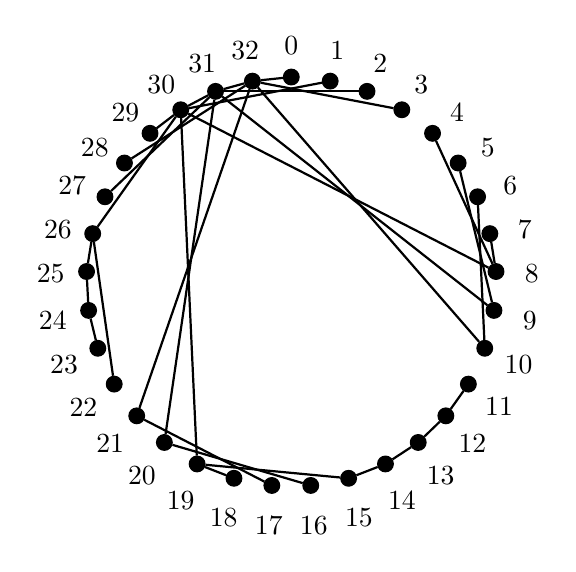
\begin{tikzpicture}
	\tikzset{enclosed/.style={draw, circle, inner sep=0pt, minimum size=0.2cm, fill=black}}

	\node[enclosed, label={above, xshift=0cm, yshift=0.052cm:0}] at (3.38, 5.2)(0){};
	\node[enclosed, label={above, xshift=0.091cm, yshift=0.039cm:1}] at (3.874, 5.148)(1){};
	\node[enclosed, label={above, xshift=0.169cm, yshift=0.013cm:2}] at (4.342, 5.018)(2){};
	\node[enclosed, label={above, xshift=0.247cm, yshift=-0.026cm:3}] at (4.784, 4.784)(3){};
	\node[enclosed, label={above, xshift=0.312cm, yshift=-0.078cm:4}] at (5.174, 4.485)(4){};
	\node[enclosed, label={above, xshift=0.377cm, yshift=-0.143cm:5}] at (5.499, 4.108)(5){};
	\node[enclosed, label={above, xshift=0.416cm, yshift=-0.208cm:6}] at (5.746, 3.679)(6){};
	\node[enclosed, label={above, xshift=0.442cm, yshift=-0.299cm:7}] at (5.902, 3.211)(7){};
	\node[enclosed, label={above, xshift=0.455cm, yshift=-0.377cm:8}] at (5.98, 2.73)(8){};
	\node[enclosed, label={above, xshift=0.455cm, yshift=-0.468cm:9}] at (5.954, 2.236)(9){};
	\node[enclosed, label={above, xshift=0.429cm, yshift=-0.546cm:10}] at (5.837, 1.755)(10){};
	\node[enclosed, label={above, xshift=0.39cm, yshift=-0.624cm:11}] at (5.629, 1.3)(11){};
	\node[enclosed, label={above, xshift=0.338cm, yshift=-0.702cm:12}] at (5.343, 0.897)(12){};
	\node[enclosed, label={above, xshift=0.286cm, yshift=-0.767cm:13}] at (4.992, 0.559)(13){};
	\node[enclosed, label={above, xshift=0.208cm, yshift=-0.806cm:14}] at (4.576, 0.286)(14){};
	\node[enclosed, label={above, xshift=0.13cm, yshift=-0.845cm:15}] at (4.108, 0.104)(15){};
	\node[enclosed, label={above, xshift=0.039cm, yshift=-0.858cm:16}] at (3.627, 0.013)(16){};
	\node[enclosed, label={above, xshift=-0.039cm, yshift=-0.858cm:17}] at (3.133, 0.013)(17){};
	\node[enclosed, label={above, xshift=-0.13cm, yshift=-0.845cm:18}] at (2.652, 0.104)(18){};
	\node[enclosed, label={above, xshift=-0.208cm, yshift=-0.806cm:19}] at (2.184, 0.286)(19){};
	\node[enclosed, label={above, xshift=-0.286cm, yshift=-0.767cm:20}] at (1.768, 0.559)(20){};
	\node[enclosed, label={above, xshift=-0.338cm, yshift=-0.702cm:21}] at (1.417, 0.897)(21){};
	\node[enclosed, label={above, xshift=-0.39cm, yshift=-0.637cm:22}] at (1.131, 1.3)(22){};
	\node[enclosed, label={above, xshift=-0.429cm, yshift=-0.546cm:23}] at (0.923, 1.755)(23){};
	\node[enclosed, label={above, xshift=-0.455cm, yshift=-0.468cm:24}] at (0.806, 2.236)(24){};
	\node[enclosed, label={above, xshift=-0.455cm, yshift=-0.377cm:25}] at (0.78, 2.73)(25){};
	\node[enclosed, label={above, xshift=-0.442cm, yshift=-0.299cm:26}] at (0.858, 3.211)(26){};
	\node[enclosed, label={above, xshift=-0.416cm, yshift=-0.208cm:27}] at (1.014, 3.679)(27){};
	\node[enclosed, label={above, xshift=-0.377cm, yshift=-0.143cm:28}] at (1.261, 4.108)(28){};
	\node[enclosed, label={above, xshift=-0.312cm, yshift=-0.078cm:29}] at (1.586, 4.485)(29){};
	\node[enclosed, label={above, xshift=-0.247cm, yshift=-0.026cm:30}] at (1.976, 4.784)(30){};
	\node[enclosed, label={above, xshift=-0.169cm, yshift=0.013cm:31}] at (2.418, 5.018)(31){};
	\node[enclosed, label={above, xshift=-0.091cm, yshift=0.039cm:32}] at (2.886, 5.148)(32){};
	\draw [thick] (0)--(32);
	\draw [thick] (8)--(4);
	\draw [thick] (8)--(7);
	\draw [thick] (9)--(5);
	\draw [thick] (10)--(6);
	\draw [thick] (12)--(11);
	\draw [thick] (13)--(12);
	\draw [thick] (14)--(13);
	\draw [thick] (15)--(14);
	\draw [thick] (19)--(15);
	\draw [thick] (19)--(18);
	\draw [thick] (20)--(16);
	\draw [thick] (21)--(17);
	\draw [thick] (24)--(23);
	\draw [thick] (25)--(24);
	\draw [thick] (26)--(22);
	\draw [thick] (26)--(25);
	\draw [thick] (30)--(1);
	\draw [thick] (30)--(8);
	\draw [thick] (30)--(19);
	\draw [thick] (30)--(26);
	\draw [thick] (30)--(29);
	\draw [thick] (31)--(2);
	\draw [thick] (31)--(9);
	\draw [thick] (31)--(20);
	\draw [thick] (31)--(27);
	\draw [thick] (31)--(30);
	\draw [thick] (32)--(3);
	\draw [thick] (32)--(10);
	\draw [thick] (32)--(21);
	\draw [thick] (32)--(28);
	\draw [thick] (32)--(31);
\end{tikzpicture}

}\\
		{\scriptsize 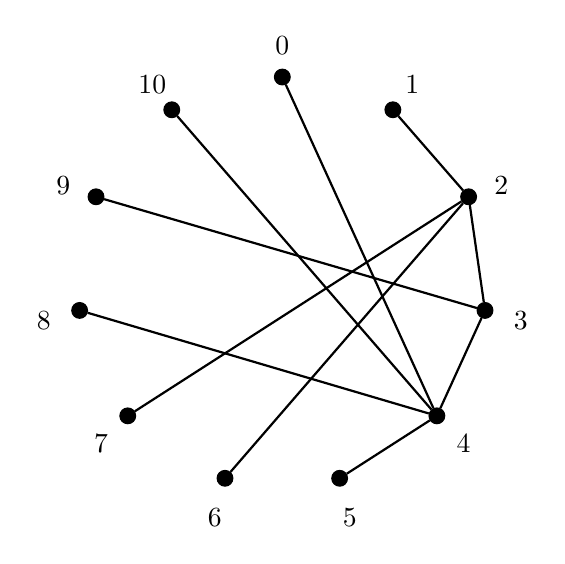
\begin{tikzpicture}
	\tikzset{enclosed/.style={draw, circle, inner sep=0pt, minimum size=0.2cm, fill=black}}

	\node[enclosed, label={above, xshift=0cm, yshift=0.052cm:0}] at (3.38, 5.2)(0){};
	\node[enclosed, label={above, xshift=0.247cm, yshift=-0.026cm:1}] at (4.784, 4.784)(1){};
	\node[enclosed, label={above, xshift=0.416cm, yshift=-0.208cm:2}] at (5.746, 3.679)(2){};
	\node[enclosed, label={above, xshift=0.455cm, yshift=-0.468cm:3}] at (5.954, 2.236)(3){};
	\node[enclosed, label={above, xshift=0.338cm, yshift=-0.702cm:4}] at (5.343, 0.897)(4){};
	\node[enclosed, label={above, xshift=0.13cm, yshift=-0.845cm:5}] at (4.108, 0.104)(5){};
	\node[enclosed, label={above, xshift=-0.13cm, yshift=-0.845cm:6}] at (2.652, 0.104)(6){};
	\node[enclosed, label={above, xshift=-0.338cm, yshift=-0.702cm:7}] at (1.417, 0.897)(7){};
	\node[enclosed, label={above, xshift=-0.455cm, yshift=-0.468cm:8}] at (0.806, 2.236)(8){};
	\node[enclosed, label={above, xshift=-0.416cm, yshift=-0.208cm:9}] at (1.014, 3.679)(9){};
	\node[enclosed, label={above, xshift=-0.247cm, yshift=-0.026cm:10}] at (1.976, 4.784)(10){};
	\draw [thick] (0)--(4);
	\draw [thick] (2)--(1);
	\draw [thick] (2)--(6);
	\draw [thick] (2)--(7);
	\draw [thick] (3)--(2);
	\draw [thick] (3)--(9);
	\draw [thick] (4)--(3);
	\draw [thick] (4)--(5);
	\draw [thick] (4)--(8);
	\draw [thick] (4)--(10);
\end{tikzpicture}

}&{\scriptsize 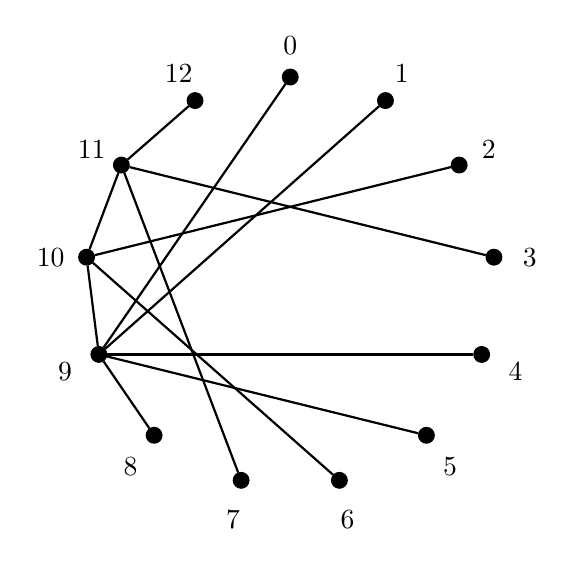
\begin{tikzpicture}
	\tikzset{enclosed/.style={draw, circle, inner sep=0pt, minimum size=0.2cm, fill=black}}

	\node[enclosed, label={above, xshift=0cm, yshift=0.052cm:0}] at (3.38, 5.2)(0){};
	\node[enclosed, label={above, xshift=0.208cm, yshift=-0cm:1}] at (4.589, 4.901)(1){};
	\node[enclosed, label={above, xshift=0.377cm, yshift=-0.143cm:2}] at (5.525, 4.082)(2){};
	\node[enclosed, label={above, xshift=0.455cm, yshift=-0.351cm:3}] at (5.967, 2.912)(3){};
	\node[enclosed, label={above, xshift=0.429cm, yshift=-0.559cm:4}] at (5.811, 1.677)(4){};
	\node[enclosed, label={above, xshift=0.299cm, yshift=-0.741cm:5}] at (5.109, 0.65)(5){};
	\node[enclosed, label={above, xshift=0.104cm, yshift=-0.845cm:6}] at (4.004, 0.078)(6){};
	\node[enclosed, label={above, xshift=-0.104cm, yshift=-0.845cm:7}] at (2.756, 0.078)(7){};
	\node[enclosed, label={above, xshift=-0.299cm, yshift=-0.741cm:8}] at (1.651, 0.65)(8){};
	\node[enclosed, label={above, xshift=-0.429cm, yshift=-0.559cm:9}] at (0.949, 1.677)(9){};
	\node[enclosed, label={above, xshift=-0.455cm, yshift=-0.351cm:10}] at (0.793, 2.912)(10){};
	\node[enclosed, label={above, xshift=-0.377cm, yshift=-0.143cm:11}] at (1.235, 4.082)(11){};
	\node[enclosed, label={above, xshift=-0.208cm, yshift=-0cm:12}] at (2.171, 4.901)(12){};
	\draw [thick] (0)--(9);
	\draw [thick] (9)--(1);
	\draw [thick] (9)--(4);
	\draw [thick] (9)--(5);
	\draw [thick] (9)--(8);
	\draw [thick] (9)--(10);
	\draw [thick] (10)--(2);
	\draw [thick] (10)--(6);
	\draw [thick] (10)--(11);
	\draw [thick] (11)--(3);
	\draw [thick] (11)--(7);
	\draw [thick] (11)--(12);
\end{tikzpicture}

}\\
		{\scriptsize 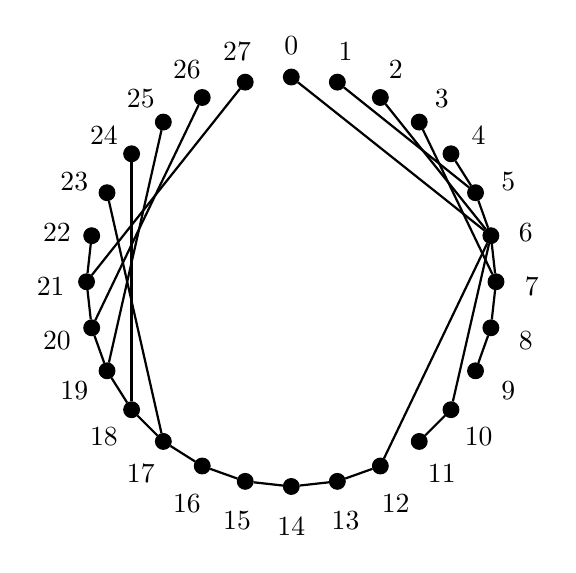
\begin{tikzpicture}
	\tikzset{enclosed/.style={draw, circle, inner sep=0pt, minimum size=0.2cm, fill=black}}

	\node[enclosed, label={above, xshift=0cm, yshift=0.052cm:0}] at (3.38, 5.2)(0){};
	\node[enclosed, label={above, xshift=0.104cm, yshift=0.039cm:1}] at (3.965, 5.135)(1){};
	\node[enclosed, label={above, xshift=0.195cm, yshift=0.013cm:2}] at (4.511, 4.94)(2){};
	\node[enclosed, label={above, xshift=0.286cm, yshift=-0.052cm:3}] at (5.005, 4.628)(3){};
	\node[enclosed, label={above, xshift=0.351cm, yshift=-0.117cm:4}] at (5.408, 4.225)(4){};
	\node[enclosed, label={above, xshift=0.416cm, yshift=-0.208cm:5}] at (5.72, 3.731)(5){};
	\node[enclosed, label={above, xshift=0.442cm, yshift=-0.299cm:6}] at (5.915, 3.185)(6){};
	\node[enclosed, label={above, xshift=0.455cm, yshift=-0.403cm:7}] at (5.98, 2.6)(7){};
	\node[enclosed, label={above, xshift=0.442cm, yshift=-0.507cm:8}] at (5.915, 2.015)(8){};
	\node[enclosed, label={above, xshift=0.416cm, yshift=-0.598cm:9}] at (5.72, 1.469)(9){};
	\node[enclosed, label={above, xshift=0.351cm, yshift=-0.689cm:10}] at (5.408, 0.975)(10){};
	\node[enclosed, label={above, xshift=0.286cm, yshift=-0.754cm:11}] at (5.005, 0.572)(11){};
	\node[enclosed, label={above, xshift=0.195cm, yshift=-0.819cm:12}] at (4.511, 0.26)(12){};
	\node[enclosed, label={above, xshift=0.104cm, yshift=-0.845cm:13}] at (3.965, 0.065)(13){};
	\node[enclosed, label={above, xshift=0cm, yshift=-0.858cm:14}] at (3.38, 0)(14){};
	\node[enclosed, label={above, xshift=-0.104cm, yshift=-0.845cm:15}] at (2.795, 0.065)(15){};
	\node[enclosed, label={above, xshift=-0.195cm, yshift=-0.819cm:16}] at (2.249, 0.26)(16){};
	\node[enclosed, label={above, xshift=-0.286cm, yshift=-0.754cm:17}] at (1.755, 0.572)(17){};
	\node[enclosed, label={above, xshift=-0.351cm, yshift=-0.689cm:18}] at (1.352, 0.975)(18){};
	\node[enclosed, label={above, xshift=-0.416cm, yshift=-0.598cm:19}] at (1.04, 1.469)(19){};
	\node[enclosed, label={above, xshift=-0.442cm, yshift=-0.507cm:20}] at (0.845, 2.015)(20){};
	\node[enclosed, label={above, xshift=-0.455cm, yshift=-0.403cm:21}] at (0.78, 2.6)(21){};
	\node[enclosed, label={above, xshift=-0.442cm, yshift=-0.299cm:22}] at (0.845, 3.185)(22){};
	\node[enclosed, label={above, xshift=-0.416cm, yshift=-0.208cm:23}] at (1.04, 3.731)(23){};
	\node[enclosed, label={above, xshift=-0.351cm, yshift=-0.117cm:24}] at (1.352, 4.225)(24){};
	\node[enclosed, label={above, xshift=-0.286cm, yshift=-0.052cm:25}] at (1.755, 4.628)(25){};
	\node[enclosed, label={above, xshift=-0.195cm, yshift=0.013cm:26}] at (2.249, 4.94)(26){};
	\node[enclosed, label={above, xshift=-0.104cm, yshift=0.039cm:27}] at (2.795, 5.135)(27){};
	\draw [thick] (0)--(6);
	\draw [thick] (5)--(1);
	\draw [thick] (5)--(4);
	\draw [thick] (6)--(2);
	\draw [thick] (6)--(5);
	\draw [thick] (6)--(7);
	\draw [thick] (6)--(10);
	\draw [thick] (6)--(12);
	\draw [thick] (7)--(3);
	\draw [thick] (7)--(8);
	\draw [thick] (8)--(9);
	\draw [thick] (10)--(11);
	\draw [thick] (12)--(13);
	\draw [thick] (13)--(14);
	\draw [thick] (14)--(15);
	\draw [thick] (15)--(16);
	\draw [thick] (16)--(17);
	\draw [thick] (17)--(18);
	\draw [thick] (17)--(23);
	\draw [thick] (18)--(19);
	\draw [thick] (18)--(24);
	\draw [thick] (19)--(20);
	\draw [thick] (19)--(25);
	\draw [thick] (20)--(21);
	\draw [thick] (20)--(26);
	\draw [thick] (21)--(22);
	\draw [thick] (21)--(27);
\end{tikzpicture}

}&{\scriptsize 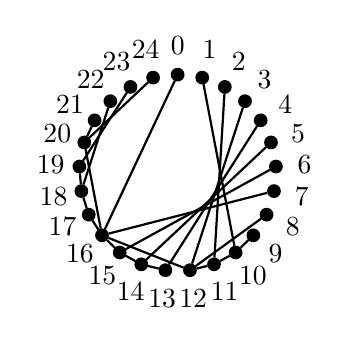
\begin{tikzpicture}[scale=0.6]
	\tikzset{enclosed/.style={draw, circle, inner sep=0pt, minimum size=0.16cm, fill=black}}

	\node[enclosed, label={above, xshift=0cm, yshift=0.0416cm:0}] at (2.704, 4.16)(0){};
	\node[enclosed, label={above, xshift=0.0936cm, yshift=0.0312cm:1}] at (3.224, 4.0976)(1){};
	\node[enclosed, label={above, xshift=0.1768cm, yshift=-0cm:2}] at (3.7024, 3.9)(2){};
	\node[enclosed, label={above, xshift=0.2496cm, yshift=-0.052cm:3}] at (4.1288, 3.5984)(3){};
	\node[enclosed, label={above, xshift=0.312cm, yshift=-0.1248cm:4}] at (4.4616, 3.1928)(4){};
	\node[enclosed, label={above, xshift=0.3432cm, yshift=-0.208cm:5}] at (4.68, 2.7248)(5){};
	\node[enclosed, label={above, xshift=0.364cm, yshift=-0.3016cm:6}] at (4.784, 2.2152)(6){};
	\node[enclosed, label={above, xshift=0.3536cm, yshift=-0.3952cm:7}] at (4.7424, 1.6952)(7){};
	\node[enclosed, label={above, xshift=0.3328cm, yshift=-0.4784cm:8}] at (4.5864, 1.196)(8){};
	\node[enclosed, label={above, xshift=0.2808cm, yshift=-0.5512cm:9}] at (4.3056, 0.7592)(9){};
	\node[enclosed, label={above, xshift=0.2184cm, yshift=-0.6136cm:10}] at (3.9312, 0.3952)(10){};
	\node[enclosed, label={above, xshift=0.1352cm, yshift=-0.6656cm:11}] at (3.4736, 0.1456)(11){};
	\node[enclosed, label={above, xshift=0.0416cm, yshift=-0.6864cm:12}] at (2.964, 0.0208)(12){};
	\node[enclosed, label={above, xshift=-0.0416cm, yshift=-0.6864cm:13}] at (2.444, 0.0208)(13){};
	\node[enclosed, label={above, xshift=-0.1352cm, yshift=-0.6656cm:14}] at (1.9344, 0.1456)(14){};
	\node[enclosed, label={above, xshift=-0.2184cm, yshift=-0.6136cm:15}] at (1.4768, 0.3952)(15){};
	\node[enclosed, label={above, xshift=-0.2808cm, yshift=-0.5512cm:16}] at (1.1024, 0.7592)(16){};
	\node[enclosed, label={above, xshift=-0.3328cm, yshift=-0.4784cm:17}] at (0.8216, 1.196)(17){};
	\node[enclosed, label={above, xshift=-0.3536cm, yshift=-0.3952cm:18}] at (0.6656, 1.6952)(18){};
	\node[enclosed, label={above, xshift=-0.364cm, yshift=-0.3016cm:19}] at (0.624, 2.2152)(19){};
	\node[enclosed, label={above, xshift=-0.3432cm, yshift=-0.208cm:20}] at (0.728, 2.7248)(20){};
	\node[enclosed, label={above, xshift=-0.312cm, yshift=-0.1248cm:21}] at (0.9464, 3.1928)(21){};
	\node[enclosed, label={above, xshift=-0.2496cm, yshift=-0.052cm:22}] at (1.2792, 3.5984)(22){};
	\node[enclosed, label={above, xshift=-0.1768cm, yshift=-0cm:23}] at (1.7056, 3.9)(23){};
	\node[enclosed, label={above, xshift=-0.0936cm, yshift=0.0312cm:24}] at (2.184, 4.0976)(24){};
	\draw [thick] (0)--(16);
	\draw [thick] (10)--(1);
	\draw [thick] (10)--(9);
	\draw [thick] (11)--(2);
	\draw [thick] (11)--(10);
	\draw [thick] (12)--(3);
	\draw [thick] (12)--(8);
	\draw [thick] (12)--(11);
	\draw [thick] (13)--(4);
	\draw [thick] (14)--(5);
	\draw [thick] (14)--(13);
	\draw [thick] (15)--(6);
	\draw [thick] (15)--(14);
	\draw [thick] (16)--(7);
	\draw [thick] (16)--(12);
	\draw [thick] (16)--(15);
	\draw [thick] (16)--(17);
	\draw [thick] (16)--(20);
	\draw [thick] (17)--(18);
	\draw [thick] (18)--(19);
	\draw [thick] (18)--(22);
	\draw [thick] (19)--(23);
	\draw [thick] (20)--(21);
	\draw [thick] (20)--(24);
\end{tikzpicture}

}\\
	\end{tabular}
	\caption{$CR(33, 4, 13)$の6つの独立全域木}
	\label{fig:CR(33, 4, 13)}
\end{figure}
